\documentclass[paper=a4, fontsize=11pt]{report} % A4 paper, 11pt font-size
\usepackage[margin=1in]{geometry} % 1 inch margin
\linespread{1} % single spacing

% --------------------
% Packages
% --------------------
\usepackage[T1]{fontenc} % Use 8-bit encoding that has 256 glyphs
\usepackage{fourier} % Use the Adobe Utopia font for the document - comment this line to return to the LaTeX default
\usepackage[english]{babel} % English language/hyphenation
\usepackage{amsmath,amsfonts,amsthm,amssymb} % Math packages
\usepackage{graphicx}
\usepackage{float} % Use [H] to force figure not float
\usepackage[section]{placeins} % prevent figures to appear in another section
\usepackage[vlined,lined,boxed,commentsnumbered]{algorithm2e}
\usepackage[colorlinks=true]{hyperref} % hyper-link
\usepackage{booktabs} % predefined table rules style
\usepackage{enumitem} % listing environment style
\usepackage{indentfirst} % indent the first line of a section
\usepackage{listings} % code listing environment
\usepackage{dirtree} % directory tree

% Font Setting
% \usepackage{fontspec}
% \setmainfont{Times New Roman}
% \setmainfont{STIXGeneral}
% \setsansfont{Arial}
% \setmonofont{Courier New}

% --------------------
% Title page
% --------------------
\title{Dell SonicWall Visualization Report}
\author{
Wanzhang Sheng\\
Kaiming Yang\\
Michelle Gao\\
Xi Han
}

% --------------------
% Document
% --------------------
\begin{document}
\maketitle


\chapter{Introduction} % (fold)
\label{cha:introduction}
% The introduction section should contain two subsections: a project overview, and a team overview. The project overview should provide a high-level description of your project, including a summary of your deliverables.
% The team overview should include a biography of each team member and your sponsor (or sponsor's company). Include details relevant to your project, including the skills and experience of each team member.
% Aim for 3 to 5 paragraphs for your project overview. There should be at least one paragraph per person in the team overview.



% chapter introduction (end)


\chapter{Specification} % (fold)
\label{cha:specification}
% The specification section should contain two subsections: functionality requirements and design. These sections should come primarily from your draft specification.
% Please see the Draft Specification assignment for additional details on what to include in these sections. Aim for 2 or more pages for this section.



% chapter specification (end)


\chapter{Implementation} % (fold)
\label{cha:implementation}
% The implementation section should contain three subsections: results, obstacles, and a timeline. The results section is where you discuss in detail your final results. The specification discusses what you wanted to complete, whereas this section discusses what you actually completed. Be specific about the functionality you implemented and the environments/tools you used.
% The obstacles section is your chance to discuss the obstacles your team encountered that slowed your progress. Discuss what happened, how you addressed the issue, and how this affected your timeline.
% The timeline section should show the actual dates you completed major milestones, and projected dates to complete the unfinished portions of your specification and test plan.
% Aim for 2 or more pages for this section.



% chapter implementation (end)


\chapter{Test Plan} % (fold)
\label{cha:test_plan}
% The test plan section should contain two subsections: objectives and scenarios. These sections should come primarily from your draft test plan.
% Please see the Draft Test Plan assignment for additional details on what to include in these sections. Aim for 2 or more pages for this section.



% chapter test_plan (end)


\chapter{Deliverables} % (fold)
\label{cha:deliverables}
% Aim for 2 or more pages for this section.

\section{Primary Deliverables} % (fold)
\label{sec:primary_deliverables}
% list the specific files containing the code you created for the primary functionality of this project.
% Include specific filenames and directory structure,
% and statistics such as the number of files, file size of these files combined, and SLOC (source-lines-of-code) for the code you provided.
% Do not include data files in this section.

Our main deliverables are our demo visualizations and the website we created for this project.

\subsection{Demo Visualizations} % (fold)
\label{sub:demo_visualizations}

\begin{description}[style=nextline]
    \item[\href{http://sjengle.cs.usfca.edu/cs690-sonicwall/public/demo/}{Dashboard}]
    Figure~\ref{fig:dashboard} aims to create a overview of the network traffic.
    We limited the result only show a summary of top ten traffic.
    It includes two parts.
    The top one is an area chart shows networking packages over time, separated by protocols.
    Users can click on it to show traffic details at the corresponding time.
    The bottom one is an sortable table. Each row indicates a different traffic by source, destination and protocol, along with a spark-line to show the trend, and a bar to show the total bytes.
    When users hover their mouse over any row, the area chart can change to the sub-dataset correspondingly.
    And also users can select a row or select multiple rows by holding command/option/shift key with a clicking to lock the dataset, then users can move their mouse to the area chart to inspect more details.
    \begin{figure}[H]
        \begin{center}
            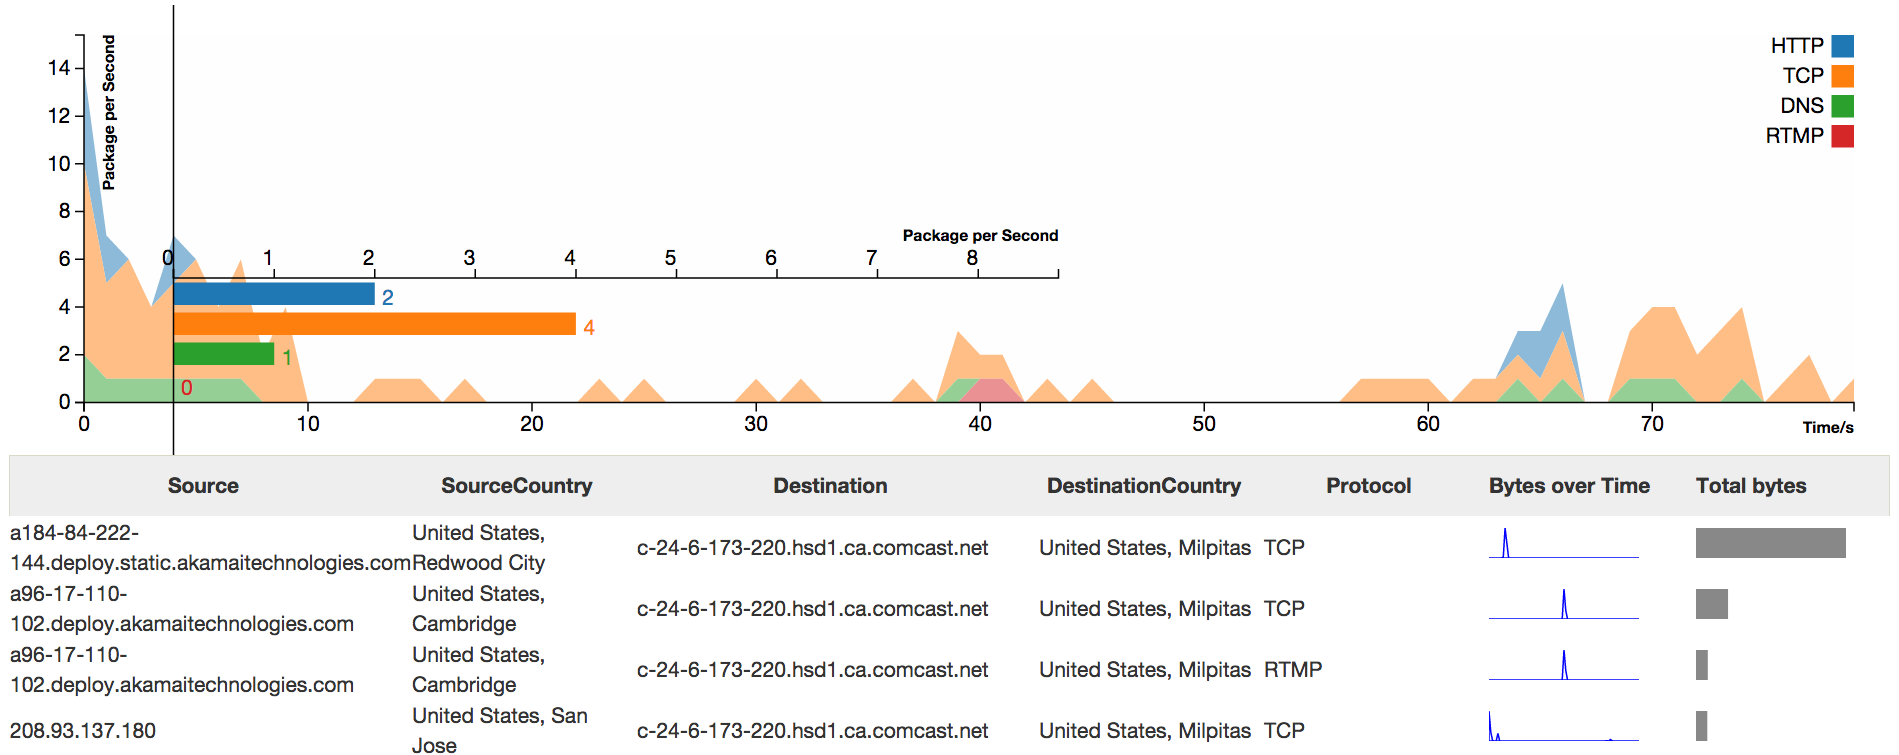
\includegraphics[width=0.9\textwidth]{dashboard.png}
        \end{center}
        \caption{Dashboard}\label{fig:dashboard}
    \end{figure}

    \item[\href{http://sjengle.cs.usfca.edu/cs690-sonicwall/wsheng/datamaps/}{Data-maps}]
    Figure~\ref{fig:datamaps} is a map visualization. It shows the traffic on a a map.
    User can switch map scope between USA and world.
    Arcs between cities indicate connections and the thickness indicates the volume.
    Circles indicate traffic volume of the cities. Cyan for source volume and red for destination volume.
    Users can toggle circles by clicking on legends.
    \begin{figure}[H]
        \begin{center}
            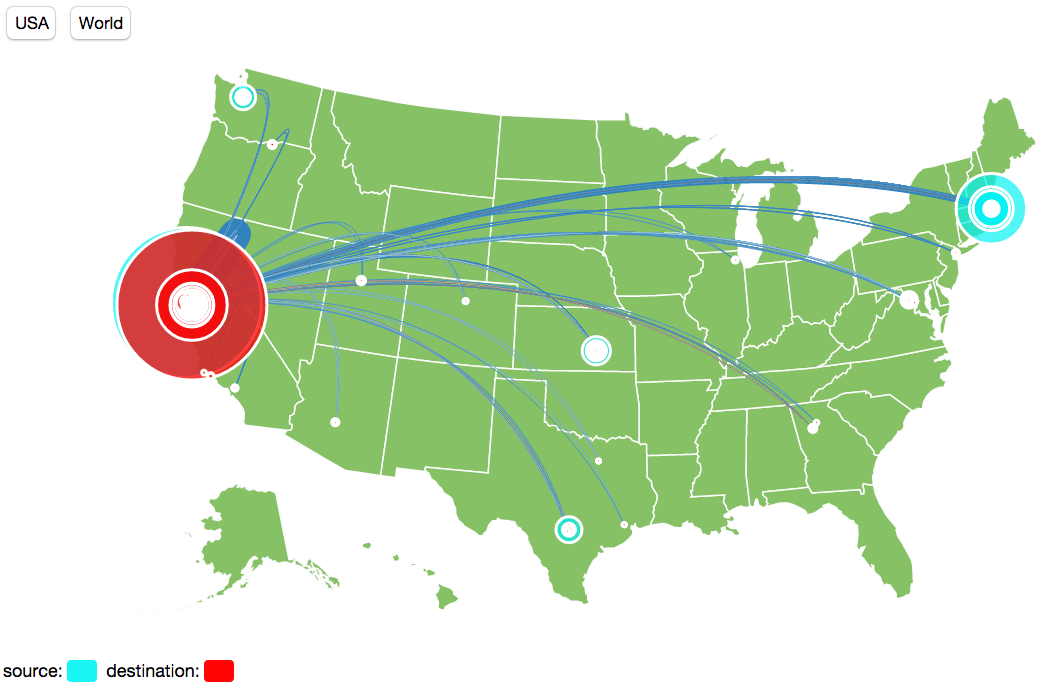
\includegraphics[width=0.9\textwidth]{datamap.png}
        \end{center}
        \caption{Data-maps}\label{fig:datamaps}
    \end{figure}

    \item[\href{http://sjengle.cs.usfca.edu/cs690-sonicwall/kyang/week-1_map_plot_refined/}{Realtime Map Plot}]
    Figure~\ref{fig:realtime} is a map visualization which keeps receiving realtime data from our back-end.
    Lines on the map indicate connections.
    By hovering on any line, users are allowed to inspect details of that connection with line charts and bar charts.
    And click to make it horizontal which make it easier to watch.
    \begin{figure}[H]
        \begin{center}
            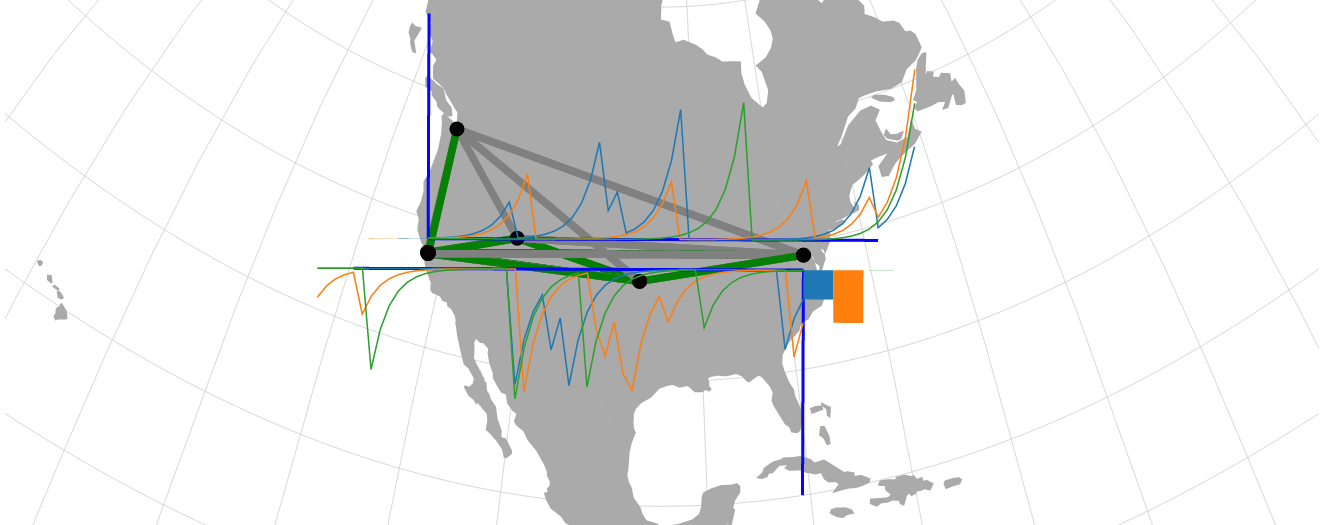
\includegraphics[width=0.9\textwidth]{realtime.png}
        \end{center}
        \caption{Realtime Map Plot}\label{fig:realtime}
    \end{figure}

\end{description}
% subsection demo_visualizations (end)

\subsection{Website} % (fold)
\label{sub:website}

Because our project is about D3 visualization, we created a website at \url{http://sjengle.cs.usfca.edu/cs690-sonicwall/} to show our work.
There are several pages on it.

\begin{description}[style=nextline]
    \item[\href{http://sjengle.cs.usfca.edu/cs690-sonicwall/}{Home}]
    This page shows a brief introduction to this project. Why we worked on this project and the basic timeline of the whole process.
    \item[\href{http://sjengle.cs.usfca.edu/cs690-sonicwall/visual.html}{Visualizations}]
    This page lists all visualizations we created for this project, including all attempts before the final visualization.
    \item[\href{http://sjengle.cs.usfca.edu/cs690-sonicwall/data.html}{Data}]
    This page shows where did we pick the data for our visualizations, and how we transformed it and mixed geography information to fit our needs.
    \item[\href{http://sjengle.cs.usfca.edu/cs690-sonicwall/tools.html}{Tools}]
    This page lists main open-source libraries or visualization tools we used during the development.
    \item[\href{http://sjengle.cs.usfca.edu/cs690-sonicwall/team.html}{Team}]
    This page lists all team members and sponsors with avatars and biographies.
\end{description}

Our works are mainly in page Visualizations.
We have seven sections indicate different attempts.
In most sections, every team member has their own attempts.
By hovering mouse on any attempt, you can see a thumbnail of the visualization.
We wished by this way, we can explore as wide as we can, to find the best way to visualize the data.

% subsection website (end)

\subsection{Directory Tree} % (fold)
\label{sub:directory_tree}

\dirtree{%
.1 /.
    .2 index.html.
    .2 visual.html.
    .2 data.html.
    .2 tools.html.
    .2 team.html.
    .2 assets/\DTcomment{Assets for pages above}.
        .3 default.css.
        .3 *.png/jpg.
    .2 public/.
        .3 prepare.rb\DTcomment{Ruby script for preparing data}.
        .3 geoip.csv\DTcomment{Geography information table}.
        .3 sfgate.csv\DTcomment{Wireshark data}.
        .3 sfgate\_summary.csv/json\DTcomment{Wireshark data summary of top 10 connections}.
        .3 sfgate\_subset.csv/json\DTcomment{Wireshark subset data with top 10 connections}.
        .3 sfgate\_with\_geoip.csv.
        .3 nsa6600/\DTcomment{SonicWall data}.
            .4 merged.csv\DTcomment{SonicWall data merged}.
        .3 demo/\DTcomment{Demo page}.
            .4 index.html.
            .4 style.css.
            .4 g1.js\DTcomment{Reusable area chart}.
            .4 table.js\DTcomment{Reusable sortable table}.
        .3 lib/.
            .4 sparkcharts/.
                .5 sparkcharts.js\DTcomment{Reusable spark chart}.
}

% subsection directory_tree (end)

\subsection{SLOC} % (fold)
\label{sub:sloc}

We use a JavaScript tool \href{https://github.com/flosse/sloc}{SLOC} to calculate source-line-of-code:

\begin{lstlisting}[language=bash, breaklines=true]
sloc . --exclude "(jquery|bootstrap|d3|p5|tip|modernizr|datamaps).*\.(js|css)|.*\.(csv|json)|nsa6600|xihan/lib"
\end{lstlisting}

This command means when it analytics files, it will exclude files which filename or pathname match the given regular expression.
By this, we remove libraries or data we used or generated in the project to make the result more meaningful and convincing.
And the result is in Table~\ref{tab:sloc}.

\begin{table}[H]
    \caption{SLOC Result}\label{tab:sloc}
    \begin{center}
        \begin{tabular}{cccccccc}
        \toprule
        \textbf{Physical} & \textbf{Source} & \textbf{Comment} & \textbf{Single-line comment} & \textbf{Block comment} & \textbf{Mixed} & \textbf{Empty} & \textbf{Number of files}\\
        \midrule
        9978     & 8226   & 621     & 384                 & 238           & 62    & 1210  & 123 \\
        \bottomrule
        \end{tabular}
    \end{center}
\end{table}

% subsection sloc (end)

% section primary_deliverables (end)

\section{Other Deliverables} % (fold)
\label{sec:other_deliverables}
% The other deliverables section should contain any data files (XML, JSON, CSV, etc.) being provided, test code, or deliverables that do not fall under another category. Include statistics for these deliverables if possible. For example, "We include ## MB of data files, and ## SLOC of test code with our project."


% section other_deliverables (end)

\section{Documentation} % (fold)
\label{sec:documentation}
% The documentation section should describe where to find documentation for your project. List the specific files that provide user documentation (for using your project), and where to find developer documentation (for extending/maintaining your project).
% If you do not provide documentation, state a strong case for why you do not provide documentation. If you do not have a strong case, you will be docked points on your final report.

% section documentation (end)

% chapter deliverables (end)


\chapter{Conclusion} % (fold)
\label{cha:conclusion}
% What we learned from this project?
% What are the shortcomings in this project?
% What can be expected to improve in the future?



% chapter conclusion (end)

\end{document}
